Per creare un progetto un utente deve essere iscritto ed autenticato. Per accedere alla pagina di creazione di un progetto l'utente deve premere il pulsante azzurro \textbf{My Project} posto in alto a destra sullo schermo. Una volta premuto si caricherà la pagina corrispondente. A questo punto l'utente deve premere il pulsante verde \textbf{New Project} posto in alto a sinistra; si aprirà un pop-up\ped{G} nel quale viene richiesto di inserire il nome del progetto che si vuole creare. Una volta inserito il nome basterà premere il pulsante \textbf{OK}.


\noindent Una volta premuto il tasto \textbf{OK} il nuovo progetto sarà creato e aggiunto alla lista dei progetti dell'utente (vedi figura sottostante).


\begin{figure}[H] 
	\centering 
	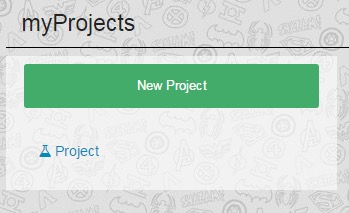
\includegraphics[scale=0.60] {img/projectlist}
	\caption{Lista dei progetti disponibili} 
\end{figure}